
\title{A NEW APPROACH TO COMPACTIFYING LOCALLY SYMMETRIC VARIETIES}
\markright{A NEW APPROACH TO COMPACTIFYING LOCALLY SYMMETRIC VARIETIES}

\author{By~ DAVID MUMFORD}
\markboth{DAVID MUMFORD}{A NEW APPROACH TO COMPACTIFYING LOCALLY SYMMETRIC VARIETIES}

\date{}
\maketitle


%\setcounter{page}{21}
\setcounter{pageoriginal}{210}

\textsc{Suppose $D$ is}\pageoriginale a bounded symmetric domain and $\Gamma \subset \Aut (D)$ is a discrete group of arithmetic type. Then Borel and Baily \cite{art8-key2} have shown that $D/\Gamma$ can be canonically embedded as a Zariski-open subset in a projective variety $\overline{D/\Gamma}$. However, Igusa  \cite{art8-key6} and others have found that the singularities of $\overline{D/ \Gamma}$ are extraordinarily complicated and this presents a significant obstacle to using algebraic geometry on $\overline{D/ \Gamma}$ in order to derive information on automorphic forms on $D$, etc. Igusa \cite{art8-key7} for $D = \fM_2$ and $\fM_3$ ($\fM_n =$ Siegel's $n \times n$ upper half-space) and $\Gamma$ commensurable with $Sp (2n ,\bZ)$, and  Hirzebruch \cite{art8-key4} for $D = \fM_1 \times \fM_1$ and $\Gamma$ commensurable with $SL(2, R)$ ($R$ = integers in a real quadratic field) have given explicit resolutions of $\overline{D/ \Gamma}$. Independently, Satake \cite{art8-key9} and I working in collaboration with Y. Tai, M. Rapaport and A. Ash have attacked the general case, using closely related methods. The purpose of this paper is to give a very short outline of my approach. It builds in an essential way on the construction of ``torus embeddings'', a theory which has been published in the Springer Lecture Notes \cite{art8-key8} (by G. Kempf, F. Knudsen, B. Saint-Donat and myself; some of which has been worked out independently by M. Demazure \cite{art8-key3} and M. Hochster \cite{art8-key5}). We intend to publish full details of the present research as soon as possible in a sequel ``Toroidal Embeddings II'' to the Notes \cite{art8-key8}. At the present time, however, we cannot claim to have written down complete proofs of our ``Main Theorem'' and although I definitely believe it is true and not difficult, it is more accurate to describe the ideas below only as a suggested approach to the problem of constructing a non-singular compactification of $D/ \Gamma$.

\section{}\label{art8-sec1}
Let us look first at the familiar case:
\begin{align*}
& D = \fM_1\\
&\Gamma = S L (2, \bZ).
\end{align*}
We know\pageoriginale that $D / \Gamma \cong \bC$ via the elliptic modular function $j$ and adding one point $j = \infty$, we get the unique non-singular compactification:
$$
\xymatrix@R=0.7cm@C=0.5cm{
D/ \Gamma \ar@{=}[d] & \subset & \overline{D / \Gamma} \ar@{=}[d]\\
\bC & \subset & \bC \bP^1
}
$$
However, let me describe a way of glueing in the point at $\infty$ that will suggest generalizations:

\begin{description}
\item[\textsc{Step} a.] Factor the $\map \fM_1 \xrightarrow{j} \bC$ as follows
$$ 
\xymatrix@R=0.7cm@C=0.5cm{
\fM_1 \ar@{=}[d] \ar[r]^{\alpha} & \Delta^\ast_1 \ar@{=}[d] \ar[r]^{\beta}& \bC\\
\{\omega | \Iim \omega > 0 \} & \{\zeta | 0 < |\zeta| < 1 \} & 
}
$$
where $\zeta = e^{2\pi i \omega}$. If $\Gamma_0 = \left\{ \left.\begin{pmatrix}1&b\\0 & 1\end{pmatrix} \right| b \in \bZ \right\}  \subset S L (2, \bZ)$, then
$$
\Delta^\ast_1 \cong \fM_1 / \Gamma_0.
$$

\item[\textsc{Step} b.] \textit{Partially} compactify $\Delta^\ast_1$ by adding the origin
$$
\Delta^\ast_1 \subset \Delta_1 = \{\zeta \big|~ |\zeta| < 1\}. 
$$

\item[\textsc{Step} c.] Note that if 
$$
\fM_1 (c) = \{\omega \big| \Iim \omega > c\},
$$
then if $c$ is large enough, $SL(2, \bZ)$-equivalence in $\fM_1$ reduces, in $\fM_1(c)$, to $\Gamma_0$-equivalence:
\begin{equation*}
\left.
\begin{aligned}
&\omega_1, \omega_2 \in \fM_1 (c) \\
&\omega_1 = \gamma (\omega_2), \; \gamma \in S L (2 , \bZ)
\end{aligned}
\right\} 
\Rightarrow \gamma \in \Gamma_0.
\tag{$\ast$}\label{art8-eq*}
\end{equation*}

Now $\fM_1 (c)$ maps to $\Delta^\ast_b$, where 
\begin{gather*}
\Delta^\ast_b = \{\zeta \big| 0< |\zeta| < b\}\\
b = e^{-2 \pi c},
\end{gather*}
and \eqref{art8-eq*} says:
$$
\res \beta : \Delta^\ast_b \to \bC \text{ is injective.}
$$

\item[\textsc{Step} d.] This gives\pageoriginale us the situation:
$$
\xymatrix@R=0.3cm@C=-0.3cm{
& &  \bC\\
&&&\\
\Delta^\ast_b \ar@{^{(}->}[uurr]_{\res \beta} \ar@{^{(}->}[ddr]& & \\
& & & \\
& (\text{Interior of closure of $\Delta^\ast_b$ in  $\Delta_1$}) = \Delta_b &
}
$$
It is easy to see that $\bC\bP^1$ is nothing but the union of $\bC$ and $\Delta_b$, glued on $\Delta^\ast_b$.
\end{description}

\section{}\label{art8-sec2}
Let us look next at how this procedure can be generalized to the $n \times n$ Siegel case:
\begin{align*}
D & = \fM_n = \left\{ \Omega \big| \Omega \;\; n \times n \text{ complex symmetric matrix,} \right.\\
& \qquad \qquad \left. \Iim \Omega \text{ positive definite} \right\},\\
\Gamma & = Sp (2n, \bZ).
\end{align*}
Actually, it is usually more convenient to replace $Sp (2n,\bZ)$ by a subgroup of finite index, or else to allow $V$-manifold-type singularities on $D/\Gamma$ and $\overline{D/\Gamma}$, because of the elements of finite order in $\Gamma$ which need not act freely. We will ignore this technicality. Of course, these $V$-manifold singularities can also be resolved: but that involves a totally different set of problems.
\begin{description}
\item[\textsc{Step} a$'$:] Factor $\fM_n \to \fM_n / \Gamma$ as follows:
$$
\xymatrix@C=0.05cm{
\fM_n \ar[r]  &\fI^0_n \ar@{=}[d] \ar[r] &  \fM_n / \Gamma\\
& \left\{ Z  \left| 
\begin{array}{l}
Z \; n \times n \text{ complex symmetric matrix, } \; Z_{ij} \neq 0 \tabularnewline
\text{and } -\log |Z_{ij}| \; \text{ positive definite}
\end{array} 
\right.
\right\} & 
}
$$
where $Z_{ij} = e^{2\pi i(\Omega_{ij})}$. If $\Gamma_0 = \left\{ \left. \begin{pmatrix}I_n & B \\ 0 & I_n \end{pmatrix}\; \right| 
\begin{array}{l}
B \in M_n (\bZ)\\
\text{and symmetric}
\end{array}
 \right\} \subset \Gamma$, then
$$
\fI^0_n \cong \fM_n /\Gamma_0.
$$

\item[\textsc{Step} b$'$:] Note that\pageoriginale $\fI^0_n$ is an open set in the algebraic torus group:
$$
\fI^0_n \subset \fI_n = 
\left\{Z \left|\begin{array}{l}
Z \; n \times n \text{ symmetric}\\
\quad Z_{ij} \neq 0
\end{array}
\right. \right\}
$$
(the group law being componentwise multiplication). The generalization of $\Delta$ in the first case is now given by the theory of equivariant torus embeddings which we must now summarize

\noindent
\textit{Torus embedding theory:}

$T$ = an algebraic torus of dimension $n, \ie, \cong (\bC^\ast)^n$,

$N$ = $\pi_1 (T)$ a free abelian group of rank $n$, $N_{\bR} = N\otimes R$, 

$N_{\bC}$ = $N \otimes \bC$ so that 

$T \cong N_{\bC} / N$ (via $\exp : N_{\bC} \to T$),

$M = \Hom (N , \bZ) \cong$ [the group of characters $\sX: T \to \bC^\ast$].

If $\alpha \in M$, write $X^\alpha: T \to \bC^\ast$ for the associated character write $\langle x, a\rangle$ for the pairing of $M_{\bR}$ and $N_{\bR}$.

$\forall \sigma$ = closed convex rational polyhedral cone in $N_{\bR}$ (\ie, $\sigma = \{\left. x \in N_{\bR} \right| \langle x, \alpha_i \rangle \geqslant 0, \; 1 \leqslant i \leqslant N\}$ for some finite set of points $\alpha_i \in M$), which are ``proper'': $\sigma \not\supset$ pos. dim subspace of $N_\bR$

$X_\sigma {}^{\;=}_{\deff} \Spec \left\{\bC [\ldots, X^\alpha, \ldots]_{\alpha\in M \cap \check{\sigma}} \right\}$, $\check{\sigma} = $ dual of $\sigma$ in $M_{\bR}$.

Then $X_\sigma$ is a normal affine variety, $T$ is an open subset of $X_\sigma$ and the action of $T$ on itself extends to an action of $T$ on $X_\sigma$; moreover all such embeddings $T \subset X$ arise like this. $X_\sigma$ is non-singular if $\sigma$ is a simplicial cone generated by a subset of a basis of $N$.
\begin{tabbing}
$\forall \{\sigma_\alpha\}$ \= = \= \;collection of such $\sigma's$ such that every face of a $\sigma_\alpha$ is\\
\> \> some $\sigma_\beta$, and every intersection $\sigma_\alpha \cap \sigma_\beta$ is a common face,\\
$X_{\{\sigma_\alpha\}}$ \> ${\displaystyle{\mathop{=}_{\deff}}} $ \> \;$\cup \;X_{\sigma_\alpha}$, where $X_{\sigma_\alpha}$ and $X_{\sigma_\beta}$ are glued along $X_{\sigma_{\alpha \cap \sigma_\beta}}$\\
\> \> (which is, in fact, an open subset of each).
\end{tabbing}
Then\pageoriginale $X_{\{\sigma_\alpha\}}$ is an irreducible separated normal scheme, locally of finite type over $\bC$, $T$ is an open subset of $X_{\{\sigma_\alpha\}}$ and the action of $T$ extends; again all such embeddings arise like this (Sumihiro \cite{art8-key10}).
\begin{tabbing}
Let \= $N_{n, \bR}$ \= = \= vector space of real $n \times n$ symmetric matrices,\\
\> $N_n$ \> = \> lattice of integral ones,\\
\> $C_n$ \> = \> cone of positive semi-definite matrices.
\end{tabbing}
Then for all collections $\{\sigma_\alpha\}$, $\sigma_\alpha \subset N_{n, \bR}$ being closed convex rational polyhedral proper cones, fitting together as above, we get
$$
\fI^0_n \subset \fI_n \subset X_{\{\sigma_\alpha\}}.
$$

It can be shown that for all $\alpha$:
$$
(\ast) 
\begin{cases}
\exists \; x \in X_{\sigma_\alpha} - \bigcup\limits_{\beta \text{ face of } \alpha} X_{\sigma_\beta}  \text{ and a neighborhood}\\
~ U \text{ of } x  \text{ in } X_{\sigma_\alpha} \text{ such that } U \subset \overline{\fI^0_n}\\
\text{ if and only if } \sigma_\alpha \subset C_n.
\end{cases}
$$

For this reason, we assume that $\sigma_\alpha  \subset C_n$, all $\alpha$, and define
$$
\fI^0_{n, \{\sigma_\alpha\}} = \text{ Interior of closure of } \fI^0_n \text{ in } X_{\{\sigma_\alpha\}}.
$$
Then 
$$
\fI^0_n \subset \fI^0_{n,\{\sigma_\alpha\}}
$$
is the partial compactification of $\fI^0_n$ which we shall use.

\item[\textsc{Step} c$'$:]  There seem to be several choices for an $n$-dimensional analog of $\fM_1(c)$ but we take:
$$
\fM_n(c) = 
\left\{\Omega \in \fM_n \left|
\begin{aligned}
&\forall \; k \in \bZ^n, \; k \neq (0), \\
& {}^t k \cdot (\Iim \Omega) \cdot k > c.
\end{aligned}
\right.
 \right\}
$$
By Siegel-Minkowski reduction theory, it can be shown that if $c$ is large enough, $Sp (2n, \bZ)$-equivalence in $\fM_n$ reduces, in $\fM_n (c)$, not to $\Gamma_0$-equivalence but to $\Gamma_1$-equivalence; where:
\begin{align*}
\Gamma_1 & = \left\{
\left. 
\begin{pmatrix}
A & B \\
0 & {}^t A^{-1}
\end{pmatrix} \;
\right|
\begin{aligned}
& A \in G L \; (n, \bZ), \; B \in M_n (\bZ) \text{ and }\\
& A^{-1} B \text{ symmetric}
\end{aligned} \right\}\\
& = \left\{
\left. 
\begin{pmatrix}
A &  B\\
0 & D
\end{pmatrix}\; 
\right|
\begin{aligned}
A, \;&  D \in G L (n, \bZ)\\
& B \in M_n (\bZ)
\end{aligned}
\cap \; Sp (2n, \bZ).
\right\}
\end{align*}
Let $\fI^0_n$ = image of $\fM_n(c)$ in $\fI_n$.

Then  $\Gamma_1 / \Gamma_0 \cong G L (n, \bZ)$\pageoriginale acts on the torus $\fI_n$, preserving the open subsets $\fI^0_n$ and $\fI^C_n$, and we get the situation:
$$
\xymatrix@R=1.2cm@C=0.05cm{
\fI^C_n \ar[d] & \subset & \fI^0_n \ar[d] & \subset & \fI_n\\
\fI^C_n / (\Gamma_1 / \Gamma_0)  \ar@{-->}[drr] & \subset & \fI^0_n / (\Gamma_1 / \Gamma_0)\ar[d] & & \\
& & \fM_n/ \Gamma & & 
}
$$
where the dotted arrow is injective.

\item[\textsc{Step} d$'$:] It is now clear how to finish up: we must assume that the collection $\{\sigma_\alpha\}$ satisfies the condition $\forall \; \gamma \in \Gamma_1 / \Gamma_0$, $\forall_\alpha$, $\exists \beta$ such that $\gamma \sigma_\alpha = \sigma_\beta$ (under the natural action of $\Gamma_1 | \Gamma_0$ on $\fI_n$, hence on $N_{n,\bR}$). Then the action of $\Gamma_1 / \Gamma_0$ on $\fI_n$ extends to $X_{\{\sigma_\alpha\}}$. Define
$$
\fI^C_{n \{\sigma_\alpha\}} = \text{ Interior of closure of } \fI^C_n \text{ in } X_{\{\sigma_{\alpha}\}} Z
$$
and consider
$$
\xymatrix{
& \fM_n/ \Gamma \\
\fI^C_n / (\Gamma_1 / \Gamma_0) \ar@{^{(}->}[ur]  \ar@{^{(}->}[dr] & \\
& \fI^C_{n, \{\sigma_\alpha\}} / (\Gamma_1/ \Gamma_0)
}
$$
and glue!

Some comments: First of all, there are many things to check in the above procedure, but we will not try to justify them here. Secondly, this glueing alone will never give us something compact;  but what I do claim is that if you take just enough $\sigma_\alpha'$s, in the sense:
\begin{itemize}
\item[(a)] $\cup \sigma_\alpha = \left\{ Z \in N_{n, \bR} \left|
\begin{aligned}
& Z \; \text{ positive semi-definite with null-}\\
& \quad \text{space defined over } \bQ
\end{aligned}
\right.
\right\}$

\item[(b)] Modulo $\Gamma_1/ \Gamma_0$, the set of $\sigma_\alpha$'s is finite,
\end{itemize} 
then the\pageoriginale resulting partial compactification of $\fM_n/\Gamma$ does cover the entire 0-dimensional boundary component: and moreover it ``analytically prolongs'' to a compactification $\overline{\fM_n/ \Gamma}$ of $\fM_n/\Gamma$  in the following way:
\begin{itemize}
\item[(a)] let 
$$
\fI^0_{n, \{\sigma_\alpha\}} = \text{ Interior of closure of } \fI^0_n \text{ in } X_{\{\sigma_\alpha\}},
$$

\item[(b)] require the existence of a map $\pi$:
$$
\xymatrix@C=0.5cm{
\fI^0_n \ar[d] & \subset &  \fI^0_{n, \{\sigma_\alpha\}} \ar@{..>}[d]^-{\pi}\\
\fM_n/\Gamma & \subset & \overline{\fM_n/\Gamma}
}
$$
where $\pi$ is surjective and open and $\fM_n/\Gamma$ is open and dense in $\overline{\fM_n/\Gamma}$.

Thirdly, the resulting space is not necessarily non-singular. However, if the $\sigma_\alpha$'s are chosen satisfying:

\item[(c)] $\forall \alpha$, $\sigma_\alpha$ is the set of positive linear combinations of matrices $A_1, \ldots, A_k \in N_n$, which are part of a basis of the free abelian group $N_n$,
\end{itemize}
and if $Sp(2n, \bZ)$ is replaced by a subgroup $\Gamma$ of finite index without elements of finite order, \textit{then} we get a non-singular compactification of $\fM_n/ \Gamma$. Even without these two conditions, the singularities are quite mild, e.g., rational (and if the $\sigma_\alpha$'s are merely simplicial cones, the singularities are $V$-manifolds). Fourthly, an objection may be raised that there is still a huge amount of freedom in the choice of the $\sigma_\alpha$'s, leading to a whole family of non-singular compactifications rather than one best possible one. This in fact discouraged me for several years and made me think the theory was not useful (the simplest case I know where this non-uniqueness seems really basic is $\fM_4$). But I believe now that this non-uniqueness is a fact of life or higher-dimensional birational geometry and that for many application, this class of compactifications is just as usable as one canonical one would be.
\end{description}

\section{}\label{art8-sec3}
Finally,\pageoriginale and with many more gaps, let me sketch how I believe this procedure extends to the general case:
\begin{align*}
D & = \text{ any bounded symmetric domain,}\\
\Gamma & = \text{ an arithmetic subgroup of $\Aut(D)$.}
\end{align*}
Assume for simplicity that $\Gamma$ has no elements of finite order.
\begin{description}
\item[\textsc{Step} a$''$.] For every rational boundary component $F$, we get groups:
$$
\Aut (D)^0 \supset N(F) \supset U (F)
$$
where
\begin{align*}
N(F) & = \left\{ g \in \Aut (D^0) \big| g^F = F \right\}\\
U(F) & = \text{center of unipotent radical of } N(F):\\
& \text{this is just a real vector space under addition.}
\end{align*}
Let $\Gamma_0 = \Gamma \cap U (F)$: a lattice in $U(F)$ and $\Gamma_1 = \Gamma \cap N (F)$.

We  factor $D \longrightarrow D / \Gamma$ via:
$$
D \longrightarrow D / \Gamma_0 \longrightarrow D/ \Gamma_1 \longrightarrow D/ \Gamma.
$$

\item[\textsc{Step} b$''$:] To describe $D$ relative to $F$ suitably, embed $D$ in $\check{D}$, its compact dual, so that the complexification $G_\bC$ of $\Aut (D)^0$ acts on $\check{D}$. Moving $D$ around only on by $U(F)_{\bC}$, we get an intermediate open set:
$$
D \subset U (F)_{\bC} \cdot D \subset \check{D}.
$$
This gives us a description of $D$ as a \textit{Siegel Domain of 3rd kind} as follows: I claim
$$
U (F)_\bC \cdot D \cong U (F)_{\bC} \times \sE (F)
$$
for some complex vector bundle $p \cdot \sE (F) \to F$ over $F$ itself (the isomorphism being complex analytic and taking the action of $U(F)_\bC$ on the left to translations in the 1st factor on the right), and that this isomorphism restricts to:
$$
D \cong \left\{(u, x) \big| \Iim u \in C (F) + h (x) \right\}
$$
for some open convex cone $C(F) \subset U (F)$ and real analytic map $h : \sE (F) \to U (F)$. Let $T (F) = U (F)_\bC/ \Gamma_0$: this is an algebraic torus group over $\bC$. We get
$$
D / \Gamma_0 \subset (U (F)_{\bC} \cdot D) / \Gamma_0 \cong T (F) \times \sE (F).
$$\pageoriginale 
We now choose a collection $\{\sigma_\alpha\}$ of rational polyhedral cones in $\overline{C(F)}$ and note that these define, by our general theory, an embedding
$$
T (F) \subset X_{\{\sigma_\alpha\}}.
$$
Define
$$
(D/\Gamma_0)_{\{\sigma_\alpha\}} = \text{ Interior of closure of } D/ \Gamma_0 in X_{\{\sigma_\alpha\}} \times \sE (F).
$$

\item[\textsc{Step} c$''$.] If $\gamma \in C(F)$ and $K \subset F$ is a compact set, let
$$
D (\gamma, K) = \Gamma_1 \cdot \left\{ (u, x) \big| \Iim  u \in C (F) + h(x) + \gamma, p(x) \in K\right\}.
$$

Then, I believe, \textit{ for all $K$, if $c$ is large enough, } the composition
$$
D(c,K) / \Gamma \hookrightarrow D / \Gamma_1 \to D / \Gamma
$$ 
is injective

\item[\textsc{Step} d$''$.] Assume now that the collection $\{\sigma_\alpha\}$ satisfies the conditions:
\begin{itemize}
\item[(a)] $\forall \gamma \in \Gamma_1 / \Gamma_0$, and $\forall \sigma_\alpha$, $\gamma \sigma_\alpha$ = some $\sigma_\beta$; and modulo this action, there are only finitely many $\sigma_\alpha's$.

\item[(b)] $C(F) \subset \bigcup\limits_\alpha \sigma_\alpha \subset \overline{C(F)}$.
\end{itemize}

It requires proof at this point that such $\{\sigma_\alpha\}$ exist --- this seems quite likely. Define
\begin{gather*}
(D(c, K)/\Gamma_0)_{\{\sigma_\alpha\}} = \text{ Interior of closure of } D (c, K)/ \Gamma_0 \text{ in }\\
X_{\{\sigma_\alpha\}} \times \sE (F)
\end{gather*}
and consider:
$$
\xymatrix{
& D/\Gamma\\
D(c, K)/\Gamma_1 \ar@{^{(}->}[ur] \ar@{^{(}->}[dr] & \\
& (D(c,K)/\Gamma_0)_{\{\sigma_\alpha\}} / (\Gamma_1/ \Gamma_0)
}
$$
and glue! The whole set-up is summarized in the figure overleaf.
\begin{figure}[H]
\centering
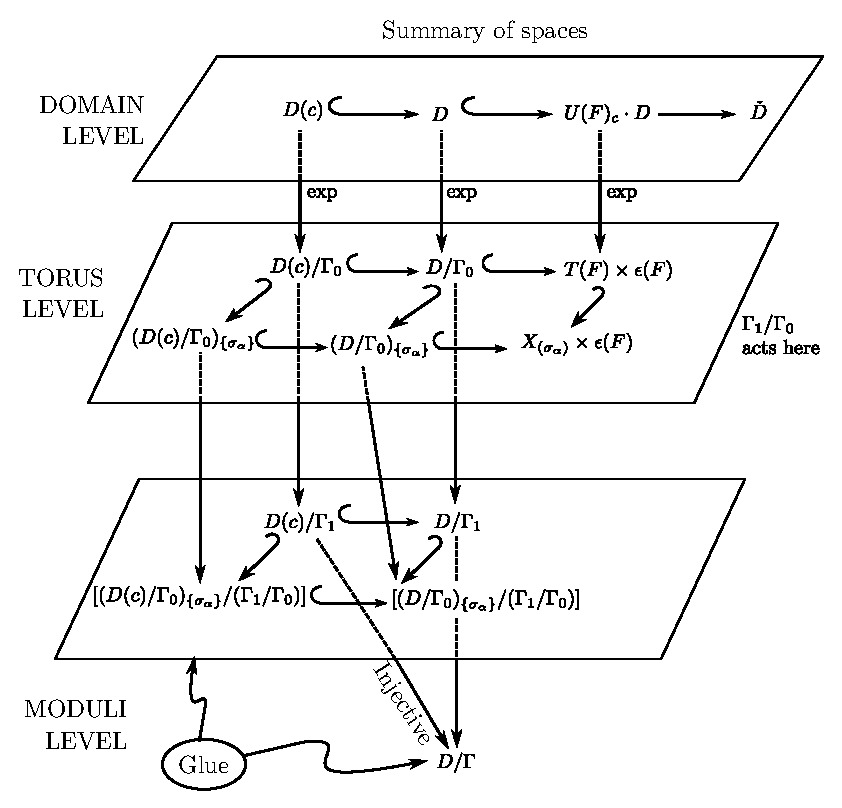
\includegraphics[scale=0.8]{220.eps}
\end{figure}

\pageoriginale
\item[\textsc{Step} e$''$.] Finally, if we let $F$ range over the finite set of $\Gamma$-inequivalent rational boundary components, we must check that if suitably compatible collections $\{\sigma_\alpha\}$ are chosen for each $F$, then these partial compactifications are compatible in the sense that they are all part of one big compact Hausdorff space $D/\Gamma$ containing $\overline{D/\Gamma}$ as an open dense set (this $D/ \Gamma$ being uniquely determined by these requirements) and such that there are even unramified maps $\pi$ in the diagram
$$
\xymatrix@R=1.2cm{
D/\Gamma_0 \ar[d]& \subset & (D/\Gamma_0)_{\{\sigma_\alpha\}} \ar@{-->}[d]^\pi\\
D/\Gamma & \subset & \overline{D/ \Gamma}
}
$$
The compatibility\pageoriginale of the $\{\sigma_\alpha\}$'s can be expressed as follows:

Say $F_1$, $F_2 \subset \overline{D}$ are 2 rational boundary components and $F_1 \subset \bar{F}_2$. Then
$$
U(F_1) \supset U (F_2) \text{~ and ~} C (F_2) \cong \text{ face of } \overline{C(F_1)}.
$$

Then we require that the set of cones $\sigma_\alpha^{(2)} \subset \overline{C(F_1)}$ be exactly the set $\sigma^{(1)}_\alpha \cap \overline{C(F_2)}$.
\end{description}

\section{}\label{art8-sec4}
In order to express more clearly what our compactification depends on, and to relate it to the theory of toroidal embeddings  (\cite{art8-key8}, Ch. II), it is convenient to introduce the following interesting abstract cone:
$$
\sum =  \left(\coprod\limits_{\substack{\text{rat. boundary}\\\text{Comp. $F$}}} C (F) \right) / \Gamma = \coprod\limits_{\substack{\text{$\Gamma$-equiv. classes}\\\text{of rat. $F$}}} (C (F) / \Gamma \cap N (F) )
$$
where $\gamma \in \Gamma$ acts on $\bigsqcup\limits_F C (F)$ by the natural maps $C(F) \xrightarrow{\approx} C(\gamma F)$ for all $F$. To express the structure that $\Sigma$ has, we use the definition.

\begin{defi*}
A `conical polyhedral complex'\footnote{This definition is a slight modification of that used in \cite{art8-key8} to allow 2 faces of the same polyhedra to be identified. Thus
\begin{figure}[H]
\centering
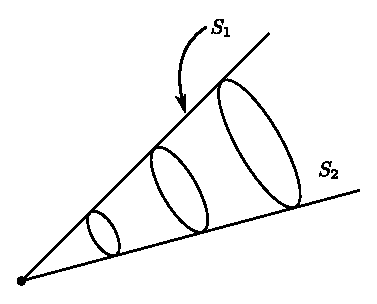
\includegraphics[scale=0.8]{221a.eps}
\end{figure}
is allowed, as well as the previously allowed:
\begin{figure}[H]
\centering
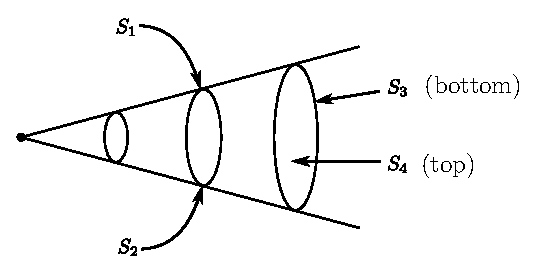
\includegraphics[scale=0.8]{221b.eps}
\end{figure}}
is a topological space $X$, plus a finite stratification $\{S_\alpha\}$ of $X$, (\ie, a partition of $X$ into disjoint locally closed pieces $S_\alpha$ such that each $\bar{S}_\alpha$ is a union of various $S_\beta$'s), plus\pageoriginale for each $\alpha$ a finite-dimensional vector-space $V_\alpha$ of real valued continuous functions on $S_\alpha$ such that :
\begin{itemize}
\item[(a)] if $n_\alpha = \dim V_\alpha$ and $f_1, \ldots, f_{n_\alpha}$ is a basis of $V_\alpha$, then $(f_i) : S_\alpha \to bR^{n_\alpha}$ is a homeomorphism of $S_\alpha$ with an open convex polyhedral cone $C_\alpha \subset \bR^{n_\alpha}$,

\item[(b)] $(f_i)^{-1}$ extends to a continuous surjective map
$$
(f_i)^{-1} : \bar{C}_\alpha  \to \bar{S}_\alpha
$$
mapping the open faces $C^{(\beta)}_\alpha$ of $\bar{C}_\alpha$ (= closed faces less their own faces) homeomorphically to the strata $S_\beta$ in $\bar{S}_\alpha$ and inducing isomorphisms
$$
\res\limits_{C^{(\beta)}_\alpha} (\text{lin. fcns.} on \bR^{n_\alpha}) \xrightarrow{\approx} V_\beta.
$$
\end{itemize}
\end{defi*}

Now for each compatible set of decompositions $\{\sigma_{\alpha, F}\}$, $\Sigma$  becomes a conical polyhedral complex: just take the $S_\alpha's$ to be the images of the sets ($\sigma_{\alpha, F}$ --- faces of $\sigma_{\alpha, F}$). In particular, this makes $\Sigma$ into a topological space with piecewise-linear structure; these structures are easily seen to be independent of the choice of $\{\sigma_{\alpha, F}\}$'s. Note that conversely, the structure $\{S_\alpha, V_\alpha\}$ of conical polyhedral complex on $\Sigma$ determines the $\{\sigma_{\alpha, F}\}'s$: they are just the closures of the connected components of the inverse images in the various $C(F)$'s of the strata $S_\alpha$. We shall call the structures $\{S_\alpha, V_\alpha\}$ on $\Sigma$ that arise from choices of $\{\sigma_{\alpha, F}\}$'s, \textit{admissible conical polyhedral subdivisions of $\Sigma$}.

Moreover $\Sigma$ has even more structure: it contains the abstract ``lattice''
$$
\Sigma_\bZ = \left(\bigsqcup\limits_F C (F) \cap \Gamma \right) /\Gamma
$$
(here regard $C(F) \subset U (F) \subset \Aut (D)^0$, so that $C(F) \cap \Gamma$ makes sense), which plays the role of the set of \textit{orders of approach to $\infty$ in $D/ \Gamma$}. In fact, let
$$
\text{R. S. } (D/\Gamma) = 
\left\{
\begin{aligned}
& \text{set of analytic maps $\varphi : \Delta^\ast \to D/\Gamma$}\\
& \text{without essential singularity at } 0 \in\Delta
\end{aligned} 
\right\}.
$$
(R. S. is short for ``Riemann surface'' as used by Zariski in higher-dimensional birational geometry). We get a natural surjective map:
$$
\text{ord } : \text{R. S. } (D/\Gamma) \to \Sigma_\bZ
$$\pageoriginale 
by the procedure: lift $\varphi$ to $\tilde{\varphi}: H \to D$, $H = \{z | \Iim z > 0\}$, such that 
$$
\tilde{\varphi} (z) \mod \Gamma = \varphi (e^{2\pi i z})
$$
hence for some $\gamma_0 \in \Gamma$:
$$
\tilde{\varphi} (z+1) = \gamma_0 \tilde{\varphi}(z), \qquad \forall_z \in H.
$$
Then $\gamma_0$ can be shown to lie in $C(F)$ for some $F$, hence it determines an element of $\Sigma_\bZ$.

We can now state the main result we hope to prove:

\begin{maintheorem*}[(?)~]
Let $D$ be a bounded symmetric domain, $\Gamma \subset \Aut D^0$ an arithmetic group without elements of finite order, and $\Sigma$ the piecewise-linear topological space defined by $D$ and $\Gamma$ as above. Then there is a map
$$
\begin{bmatrix}
\text{ Admissible conical }\\
\text{ polyhedral subdivisions }\\
\{S_\alpha, V_\alpha\} \text{ of } \Sigma
\end{bmatrix} 
\longmapsto
\begin{bmatrix}
\text{ toroidal embeddings }\\
\text{ $D/ \Gamma \subset \overline{D/ \Gamma}$, where }\\
\text{ $\overline{D/ \Gamma}$ is a compact }\\
\text{ algebraic space }
\end{bmatrix}
$$
such that if $\Sigma (\overline{D/\Gamma})$ is the conical polyhedral complex associated by the theory in \cite{art8-key8} to this toroidal embedding\footnote{In general, $D/\Gamma \subset \overline{D/\Gamma}$ may be a toroidal embedding with self-intersection, however, it is without twisting in the sense that for all strata $T$, the branches of $\overline{D/\Gamma}-D/\Gamma$ through $T$ are no permuted by going around loops in $T$. This makes it possible to associate a complex of the type defined above to this embedding by a generalization of the procedure in (\cite{art8-key8}, Ch. II).}, there is a unique isomorphism $\varphi$ making the diagram
$$
\xymatrix{
& \Sigma\ar[dd]^\varphi_{\approx}\\
R. S. (D/ \Gamma) \ar[ur]^{\text{ord}}\ar[dr]_{\text{ord}}& \\
& \Sigma (\overline{D/\Gamma})
}
$$
commute.\pageoriginale The map is a functor in the sense that if (subd)$_1$ is finer than (subd)$_2$, then $(\overline{D/\Gamma})^{(1)}$ dominates $(\overline{D/\Gamma})^{(2)}$. An integrality condition on the subdivision $\{S_\alpha, V_\alpha\}$ characterize which $\overline{D/\Gamma}$'s are non-singular (see p. 11 above).
\end{maintheorem*}

I also expect that certain convexity properties of the subdivision imply $\overline{D/\Gamma}$ projective.

\begin{thebibliography}{99}
\bibitem{art8-key1} \textsc{M. Artin :} Algebraic Spaces, \textit{Yale Math. Monographs.}

\bibitem{art8-key2} \textsc{A. Borel} and \textsc{W. Baily :} Compactification of arithmetic quotients of bounded symmetric domains, \textit{Annals of Math.,} 84 (1966), 442-528.

\bibitem{art8-key3} \textsc{M. Demazure:} Sous-groups alg\'ebriques des rang maximum du groupe de Cremona, \textit{Annales de ENS,} 3 (1970).

\bibitem{art8-key4}  \textsc{F. Hirzebruch:} Hilbert modular surfaces, \textit{L'Enseigement Math.} (1973).

\bibitem{art8-key5}  \textsc{M. Hochster:} Rings of invariants of tori, Cohen-Macauley rings generated by monomials and polytopes, \textit{Annals of Math.} 96, (1972).

\bibitem{art8-key6}  \textsc{J.-I. Igusa:} On the desingularization of Satake compactifications in Algebraic Groups, \textit{Proc. of AMS Symposia in Pure Math.,} vol. 9, (1966).

\bibitem{art8-key7}  \textsc{J.-I. Igusa:} A desingularization problem in the theory of Siegel modular functions, \textit{Math. Annalen}, 168 (1967), 228-260.

\bibitem{art8-key8}  \textsc{G. Kempf, F. Knudsen, D. Mumford} and \textsc{B. Saint-Donat:} Toroidal Embeddings I, \textit{Springer Lecture Notes,} 339, (1973).

\bibitem{art8-key9}  \textsc{I. Satake:} One the arithmetic of tube domains, \textit{Bull. Amer. Math. Soc.}, 79(1973), 1076.

\bibitem{art8-key10}  \textsc{H. Sumihiro:} Equivariant Completion, \textit{Kyoto Math. J.,} 14, (1974).
\end{thebibliography}

